\documentclass[10.5pt,a4paper]{article}
\usepackage{fontspec}
\usepackage{polyglossia}
\setdefaultlanguage{turkish}
\setmainfont{TeX Gyre Pagella}
\setmonofont{DejaVu Sans Mono}[Scale=0.85]
\usepackage[a4paper,margin=2cm]{geometry}
\usepackage{graphicx,booktabs,float,caption,xcolor,enumitem,amsmath,microtype,fancyhdr,array,tabularx}
\usepackage[hidelinks]{hyperref}
\captionsetup{font=small,labelfont=bf,labelsep=period}
\captionsetup[table]{position=top}
\setlist{nosep,leftmargin=1.3em}
\graphicspath{{../figures/}}
\pagestyle{fancy}\fancyhf{}\rhead{\small MLP ile Sınıflandırma ve Nested CV}\lhead{\small Yapay Sinir Ağları Ara Sınav Projesi}\cfoot{\thepage}
\renewcommand{\arraystretch}{1.12}
\newcommand{\tbl}[1]{\input{tables/#1}}
\setlength{\parskip}{3pt}
\setlength{\emergencystretch}{3em}

\begin{document}
\begin{titlepage}
\centering\vspace*{3cm}
{\Large YAPAY SİNİR AĞLARI DERSİ\\[4pt] YÜKSEK LİSANS ARA SINAV PROJESİ\par}\vspace{1.6cm}
{\LARGE\bfseries MLP ile Sınıflandırma: EDA, Ön İşleme,\\[4pt] Hiperparametre Optimizasyonu ve Nested Cross-Validation\par}\vspace{1.2cm}
{\large UCI Bank Marketing veri seti (bank-additional.csv) üzerinde teknik rapor\par}\vspace{2.2cm}
{\large Hazırlayan: İbrahim Alpsoy\\[3pt] Öğrenci No: 254329040\par}\vspace{0.8cm}
{\large Öğretim Üyesi: Doç. Dr. Gökalp Tulum\par}\vspace{1.2cm}
\begin{tabular}{ll}
Temel seed & 29040 + 2026 = 31066\\
Yazılım & Python 3.13, PyTorch 2.15, scikit-learn 1.9\\
GitHub & \url{https://github.com/ibrahimalpsoy/ysa-midterm-bank-mlp}\\
\end{tabular}
\vfill {\large Kasım 2026\par}
\end{titlepage}

\section*{Özet}
Araştırma sorusu: MLP modelinin başarısı ön işleme, mimari, optimizer ve eğitim ayarlarına ne kadar bağlı ve bu ayarlar sızıntısız bir nested CV ile seçildiğinde model yeni veride ne kadar başarılı oluyor?
UCI Bank Marketing veri setinin bank-additional.csv dosyasında (4119 gözlem, pozitif oran yaklaşık \%11) müşterinin vadeli mevduata abone olup olmayacağını PyTorch ile yazdığım bir MLP ile tahmin ettim.
duration değişkenini görüşmeden önce bilinmediği için çıkardım. Veriyi \%80 development ve \%20 test olarak ayırdım, development üzerinde 3x3 nested CV kurdum ve 6 manuel ile 6 random search adayını Average Precision (AP) ile karşılaştırdım.
Dış CV AP sonuçları manuel arama için 0.422 ± 0.061, random search için 0.405 ± 0.044, lojistik regresyon için 0.414 ± 0.061 ve Dummy için 0.110 oldu.
Seçilen R5 modeli (AdamW, 16 nöron, tanh, dropout 0.2) kilitli test setinde 0.440 AP (\%95 CI 0.336-0.561) ve 0.784 ROC-AUC verdi.
MLP ile lojistik regresyon arasındaki fark anlamlı çıkmadı.

\section{Giriş}
MLP, girdiyi doğrusal katmanlar ve aktivasyon fonksiyonlarından geçirerek doğrusal olmayan karar sınırları öğrenebilir. Bu esneklik yüzünden başarısı öğrenme oranı, optimizer, mimari, ölçekleme ve düzenlileştirme gibi seçimlere bağlıdır.
Hiperparametreler aynı veride hem seçilip hem değerlendirilirse skor olduğundan iyi görünür. Bu yüzden nested CV kullandım: iç döngü hiperparametreyi seçiyor, dış döngü bu seçim sürecinin başarısını ölçüyor.
Veride pozitif sınıf \%11 civarında. Her müşteriye hayır diyen bir model bile \%89 accuracy alacağı için ana metrik olarak AP kullandım. AP için şans seviyesi pozitif oran kadardır (yaklaşık 0.11).

\section{Veri Seti ve Keşifsel Veri Analizi}
\subsection{Veri, kurallar ve bölünme}
Sütun adlarını, tipleri ve hedef etiketleri kontrol ettikten sonra model sonuçlarına bakmadan şu kuralları belirledim: duration çıkarıldı, yes 1 ve no 0 olarak kodlandı, unknown NaN sayılmadı ve ayrı kategori olarak tutuldu, pdays = 999 daha önce aranmamış müşteriyi gösterdiği için silinmedi.
Sonra stratified \%80 / \%20 bölünme yaptım (seed 31069) ve satır indekslerini results/dataset\_split.csv dosyasına kaydettim (Tablo 1).
Ham veride kopya yok. duration çıkarılınca 19 satır birebir aynı hale geliyor. Müşteri numarası olmadığı için bunların aynı kişi mi farklı kişiler mi olduğu bilinemiyor, bu yüzden silmedim. Development içinde aynısı olan test satırı sayısı 5 (testin \%0.6 kadarı).
Rastgele bölünme yeni müşterilere veya ileriki dönemlere genellemeyi tam göstermez, çünkü kayıtlar 2008-2010 kampanyalarından geliyor ve aynı döneme ait ekonomik göstergeler hem eğitimde hem testte var.

\begin{table}[H]\centering\caption{Veri seti, sınıf dağılımı ve eksik veya özel kodlu değerler. Değerleri 01\_eda.ipynb içinde hesapladım (results/eda\_feature\_overview.csv, split\_summary.csv, duplicate\_report.json).}\label{tab:data}\small\tbl{t1a_dataset}\end{table}

\begin{figure}[H]\centering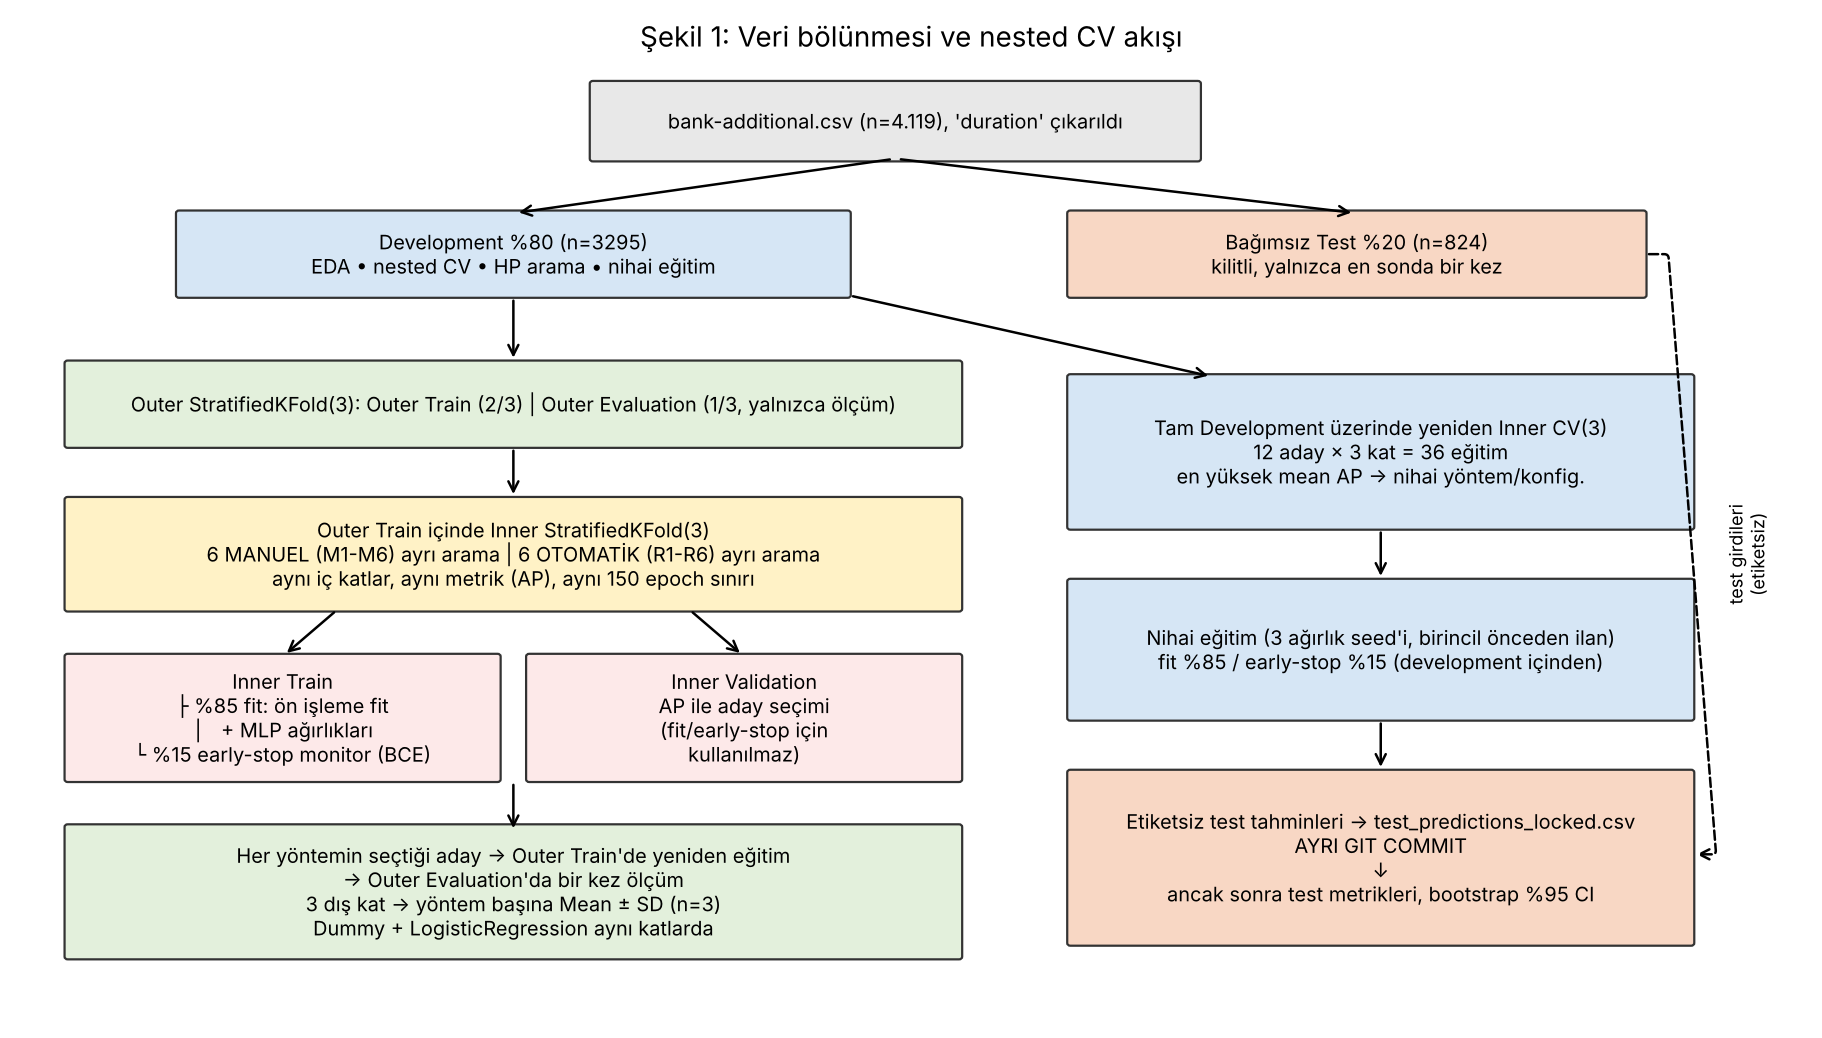
\includegraphics[width=.78\linewidth]{fig01_nested_cv_flow.png}
\caption{Veri bölünmesi ve nested CV akışı. Şemayı 02\_nested\_cv.ipynb içinde matplotlib ile çizdim.}\label{fig:flow}\end{figure}

\subsection{Development verisinde EDA}
EDA sadece development verisinde (3295 satır) yapıldı (Tablo 2, Şekil 2a). campaign sağa çarpık ve verinin \%6 kadarı IQR üst sınırının üstünde. previous değerlerinin \%86 kadarı sıfır. pdays değerlerinin \%96 kadarı 999.
Ekonomik değişkenler az sayıda farklı değer alıyor ve emp.var.rate, euribor3m, nr.employed arasındaki korelasyon 0.89 üstünde (Şekil 2b).
unknown oranı en çok default (\%19.1) ve education (\%4.4) değişkenlerinde (Şekil 2c). default = yes sadece 1 kez geçtiği için one-hot sonrası girdi sayısı katlara göre 62 veya 63 oluyor.
Abone olanlarda euribor3m medyanı 1.26, olmayanlarda 4.86. Önceki kampanyası başarılı olanlarda abone olma oranı \%63.7.
Bu karşılaştırmalar sadece betimsel. Bunlara göre özellik seçmedim çünkü bu da model seçimi sayılır. Aykırı değerleri IQR ve \%1-\%99 sınırlarıyla işaretledim ama silmedim, bunun yerine eğitim katında öğrenilen kırpmayı random search içine seçenek olarak ekledim.

\begin{table}[H]\centering\caption{Sayısal değişkenlerin tanımlayıcı istatistikleri (development, SD örnek standart sapması). 01\_eda.ipynb içinde pandas ile hesapladım (results/eda\_numeric\_descriptives.csv).}\label{tab:num}\small\tbl{t1b_numeric}\end{table}

\setcounter{figure}{1}\renewcommand{\thefigure}{2a}
\begin{figure}[H]\centering
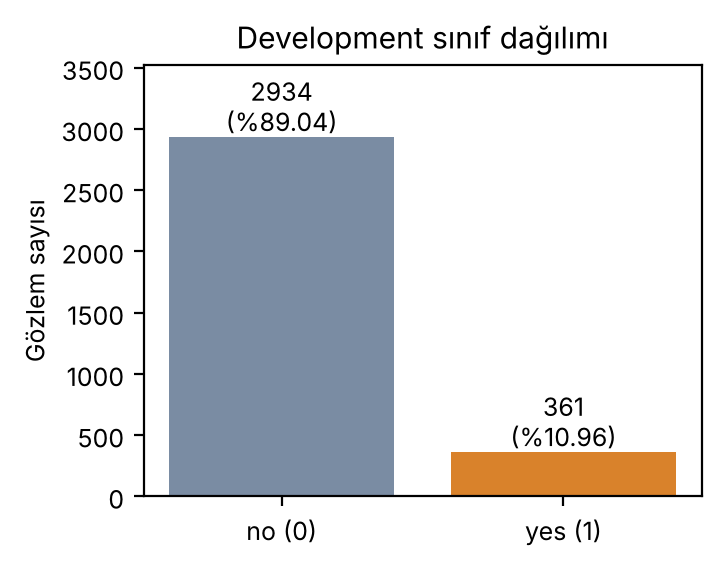
\includegraphics[width=.3\linewidth]{fig02a_class_distribution.png}\\[4pt]
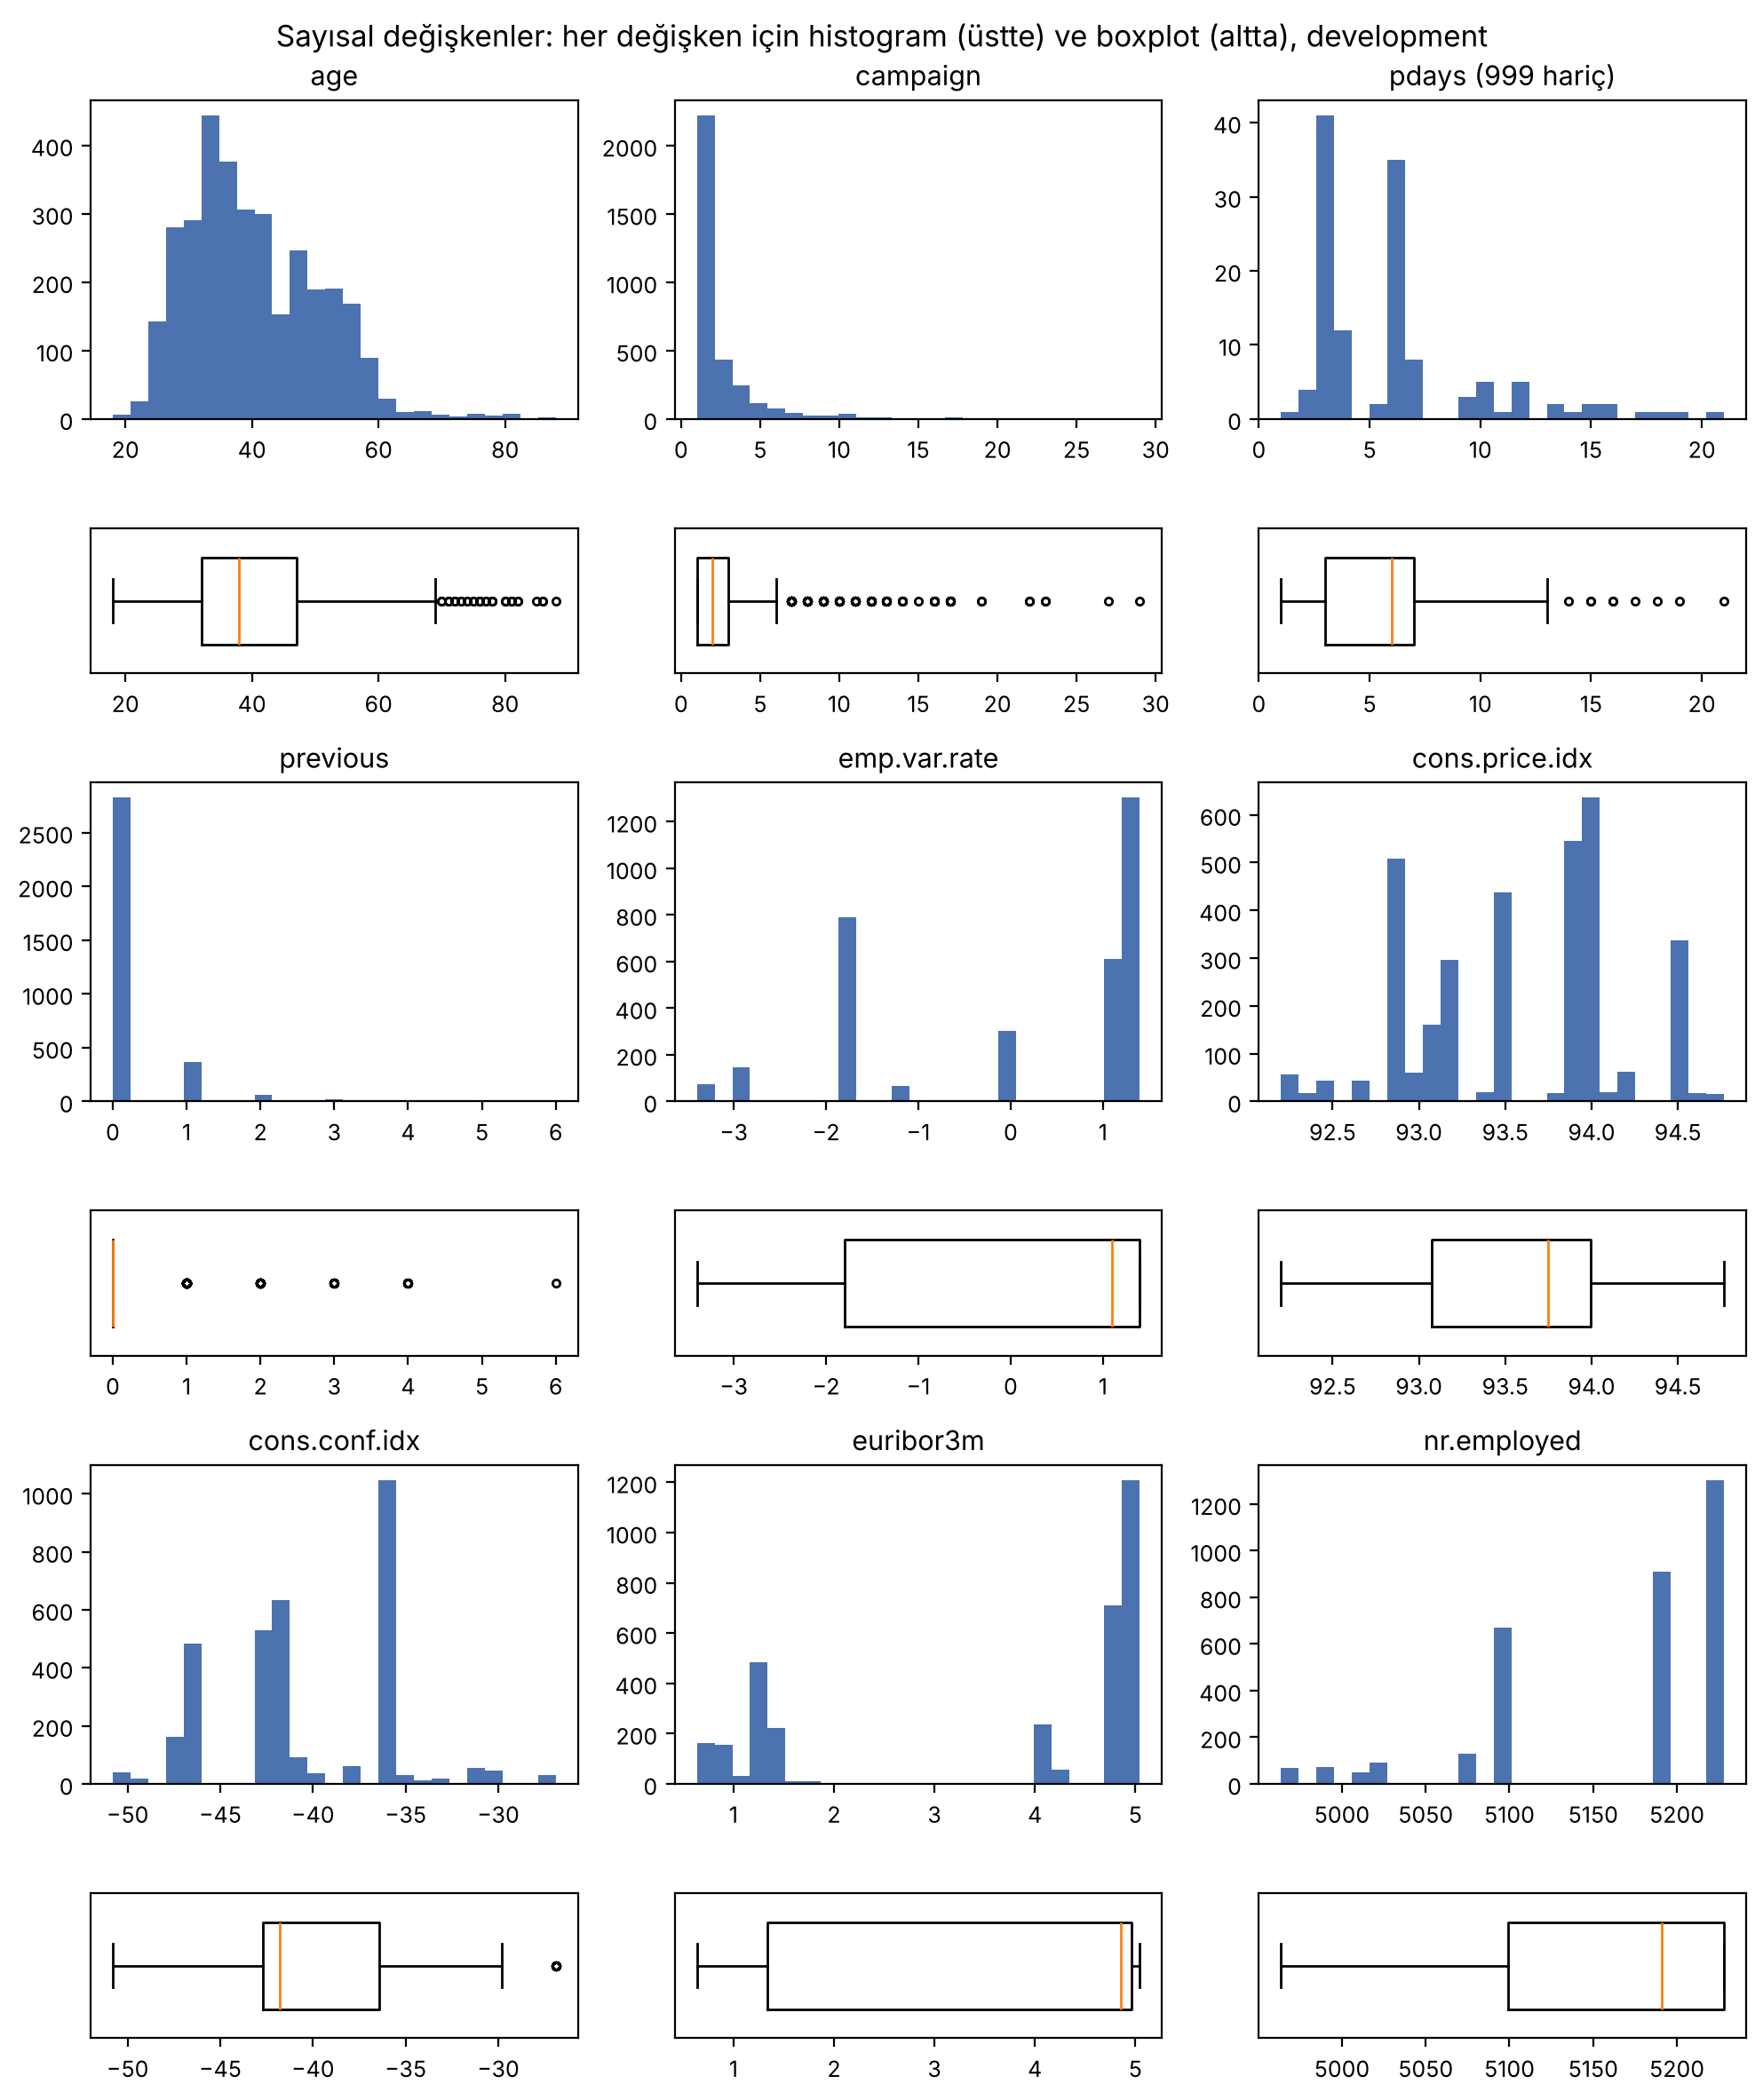
\includegraphics[width=.74\linewidth]{fig02b_numeric_hist_box.png}
\caption{Sınıf dağılımı (üstte) ve sayısal değişkenlerin histogram ve boxplot grafikleri (altta). pdays için 999 olmayan değerler çizildi. Grafikleri 01\_eda.ipynb içinde development verisinden matplotlib ile çizdim.}\label{fig:eda}\end{figure}
\renewcommand{\thefigure}{2b}
\begin{figure}[H]\centering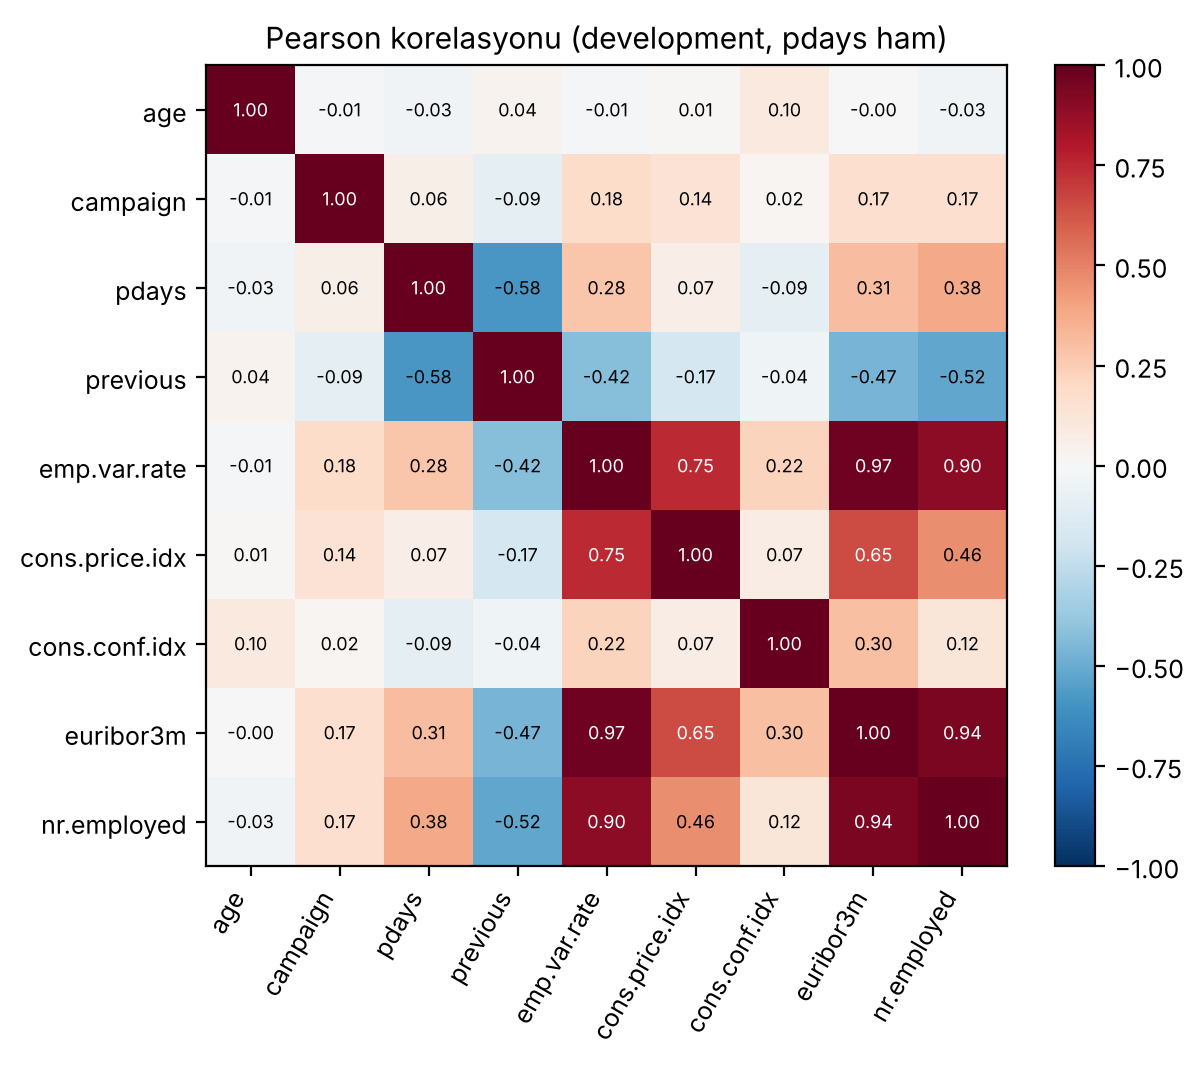
\includegraphics[width=.55\linewidth]{fig02d_correlation.png}\caption{Sayısal değişkenler için Pearson korelasyon matrisi. 01\_eda.ipynb içinde pandas corr() ile hesaplayıp çizdim.}\label{fig:corr}\end{figure}
\renewcommand{\thefigure}{2c}
\begin{figure}[H]\centering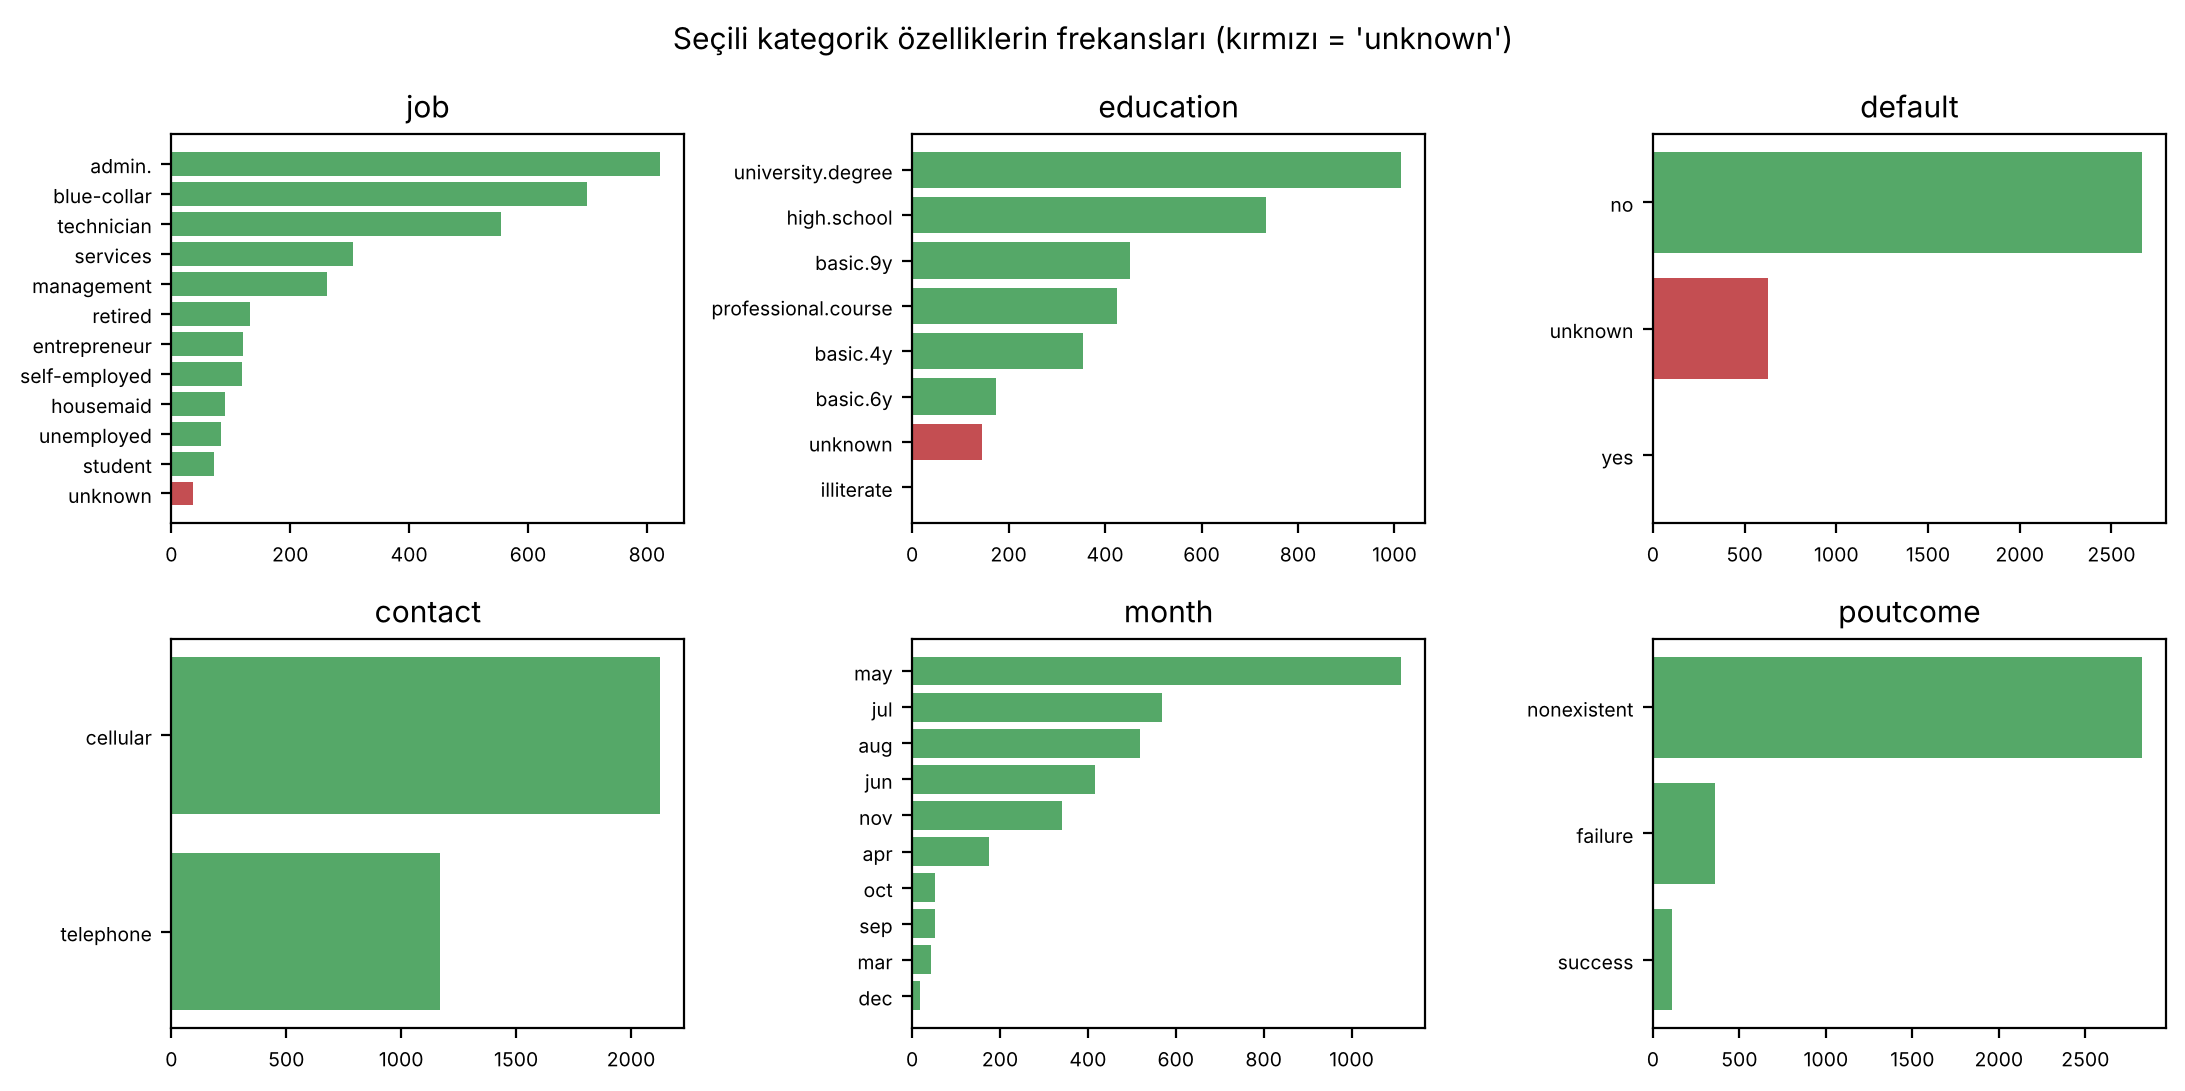
\includegraphics[width=.8\linewidth]{fig02c_categorical_bars.png}\caption{Bazı kategorik değişkenlerin frekansları (kırmızı olanlar unknown). 01\_eda.ipynb içinde development verisinden çizdim.}\label{fig:cat}\end{figure}
\renewcommand{\thefigure}{\arabic{figure}}\setcounter{figure}{2}

\subsection{Deney hipotezleri}
Nested CV çalıştırılmadan önce configs/hypotheses.md dosyasına yazıldı:
\begin{itemize}
\item H1: Öğrenme oranı 0.001 iken SGD (M3), AdamW (M1) modelinden yavaş öğrenir ve daha iyi olmaz. Adam ile AdamW farkı küçüktür.
\item H2: Çarpık değişkenler yüzünden MinMax (M4), StandardScaler (M1) modelinden iyi olmaz.
\item H3: Daha büyük (64,32) mimarisi (M5) belirgin kazanç sağlamaz ve daha erken aşırı öğrenir.
\item H4: Early stopping açıkken scheduler kapatılırsa (M6) AP pek değişmez.
\item H5: En iyi MLP ile lojistik regresyon farkı 0.03 AP altında kalır ve ikisi de Dummy modeli geçer.
\end{itemize}

\section{Yöntem}
\subsection{Seed ve deney akışı}
Temel seed 29040 + 2026 = 31066. Diğer seedleri buna sabit sayılar ekleyerek ürettim: Python 31066, NumPy 31067, PyTorch 31068, bölünme 31069, dış CV 31070, iç CV 31071, random search 31072, early stopping bölünmesi 31073, bootstrap 31074. Final model için ağırlık seedleri 31068 (ana), 31166 ve 31266. PyTorch deterministik modda, CPU üzerinde çalıştırıldı.

Dış döngüde 3 katlı StratifiedKFold ile development verisi outer train ve outer evaluation olarak ayrıldı. Outer train içinde 3 katlı iç CV yapıldı ve 6 manuel ile 6 random aday iki ayrı arama olarak aynı iç katlarda denendi (Şekil 1).
Her iç eğitimde inner train verisi ayrıca bölündü: \%85 fit alt kümesinde ön işleme parametreleri öğrenildi ve ağırlıklar güncellendi, \%15 kısımda early stopping ve scheduler için BCE kaybı izlendi. İç validation katı sadece AP hesaplamak için kullanıldı.
Her yöntemde iç CV ortalama AP değeri en yüksek aday seçildi, outer train üzerinde tekrar eğitildi ve outer evaluation üzerinde bir kez ölçüldü. Dış skorlar adayları değiştirmek veya son modeli seçmek için kullanılmadı.
Son seçim için iç CV tüm development verisinde tekrar çalıştırıldı, en iyi aday 3 seed ile eğitildi. Test tahminleri etiketlere bakılmadan ayrı bir commit ile kaydedildi (d463f75), test metrikleri bundan sonra hesaplandı.
Toplamda 108 iç eğitim, 6 dış eğitim, 36 son seçim eğitimi ve 3 final eğitim yapıldı.

\subsection{Katlar içinde ön işleme}
Ön işleme scikit-learn Pipeline ve ColumnTransformer ile yapıldı. Fit sadece ilgili eğitim alt kümesinde yapıldı, diğer kümelere sadece transform uygulandı.
pdays için prev\_contacted (daha önce arandı mı) değişkeni eklendi, 999 değerleri NaN yapılıp eğitim katı medyanı ile dolduruldu. Sayısal değişkenlere medyan ile doldurma, istenirse \%1-\%99 kırpma ve ölçekleme uygulandı. Kategorik değişkenler için \texttt{OneHotEncoder(handle\_unknown="ignore")} kullanıldı.
Normalization ile standardization farklıdır: StandardScaler z = (x - ortalama) / standart sapma ile ortalamayı 0 ve varyansı 1 yapar, aralığı sınırlamaz. MinMaxScaler (x - min) / (max - min) ile değerleri 0-1 arasına getirir ve uç değerlerden etkilenir. RobustScaler medyan ve IQR kullandığı için aykırı değerlere daha dayanıklıdır.
Final modelde öğrenilen istatistikler final\_hyperparameters.json dosyasına kaydedildi.

\subsection{Kod ve çıktıların üretilmesi}
Kodun ortak kısımlarını src klasöründe yazdım (veri okuma, ön işleme, MLP, nested CV ve metrikler) ve notebooklardan bu fonksiyonları çağırdım. Raporda kullandığım bütün grafikleri 01, 02 ve 03 notebooklarında matplotlib ile çizdim. Tabloları ise elle yazmak yerine results klasöründeki CSV dosyalarından, report klasöründeki make\_tables.py betiği ile LaTeX tablosuna çevirdim. Böylece rapordaki sayılar doğrudan çalıştırdığım deneylerin çıktılarıyla aynı.

\subsection{MLP yapısı, eğitim ve referans modeller}
MLP her gizli katmanda Linear, aktivasyon ve gerekirse Dropout içeriyor, son katman tek logit veriyor. Kayıp BCEWithLogitsLoss, olasılık sigmoid ile hesaplanıyor.
Parametre sayısı her katman için (girdi + 1) x çıktı formülüyle bulunuyor. 63 girdili (32,) modelde 64 x 32 + 33 = 2081 parametre var (Şekil 3).
En fazla 150 epoch eğitildi. Early stopping patience 15 ile en iyi ağırlıkları geri yükledi. ReduceLROnPlateau factor 0.5, patience 5, min\_lr 0.00001 ile her epoch sonunda early stopping kümesindeki BCE kaybına göre güncellendi.
Early stopping için AP yerine BCE kullandım çünkü küçük izleme kümesinde (yaklaşık 50 pozitif) AP çok dalgalanıyor. Hiperparametre seçiminde ana metrik AP. SGD momentum 0.9, eşik 0.50. Epoch bazında kayıplar, öğrenme oranı, en iyi epoch, süre ve uyarılar CSV olarak kaydedildi.
Referans olarak DummyClassifier (prior) ve sabit ön işlemeli LogisticRegression (C = 1) kullandım. İkisi de dış katlarda sadece outer train ile eğitildi.

\begin{figure}[H]\centering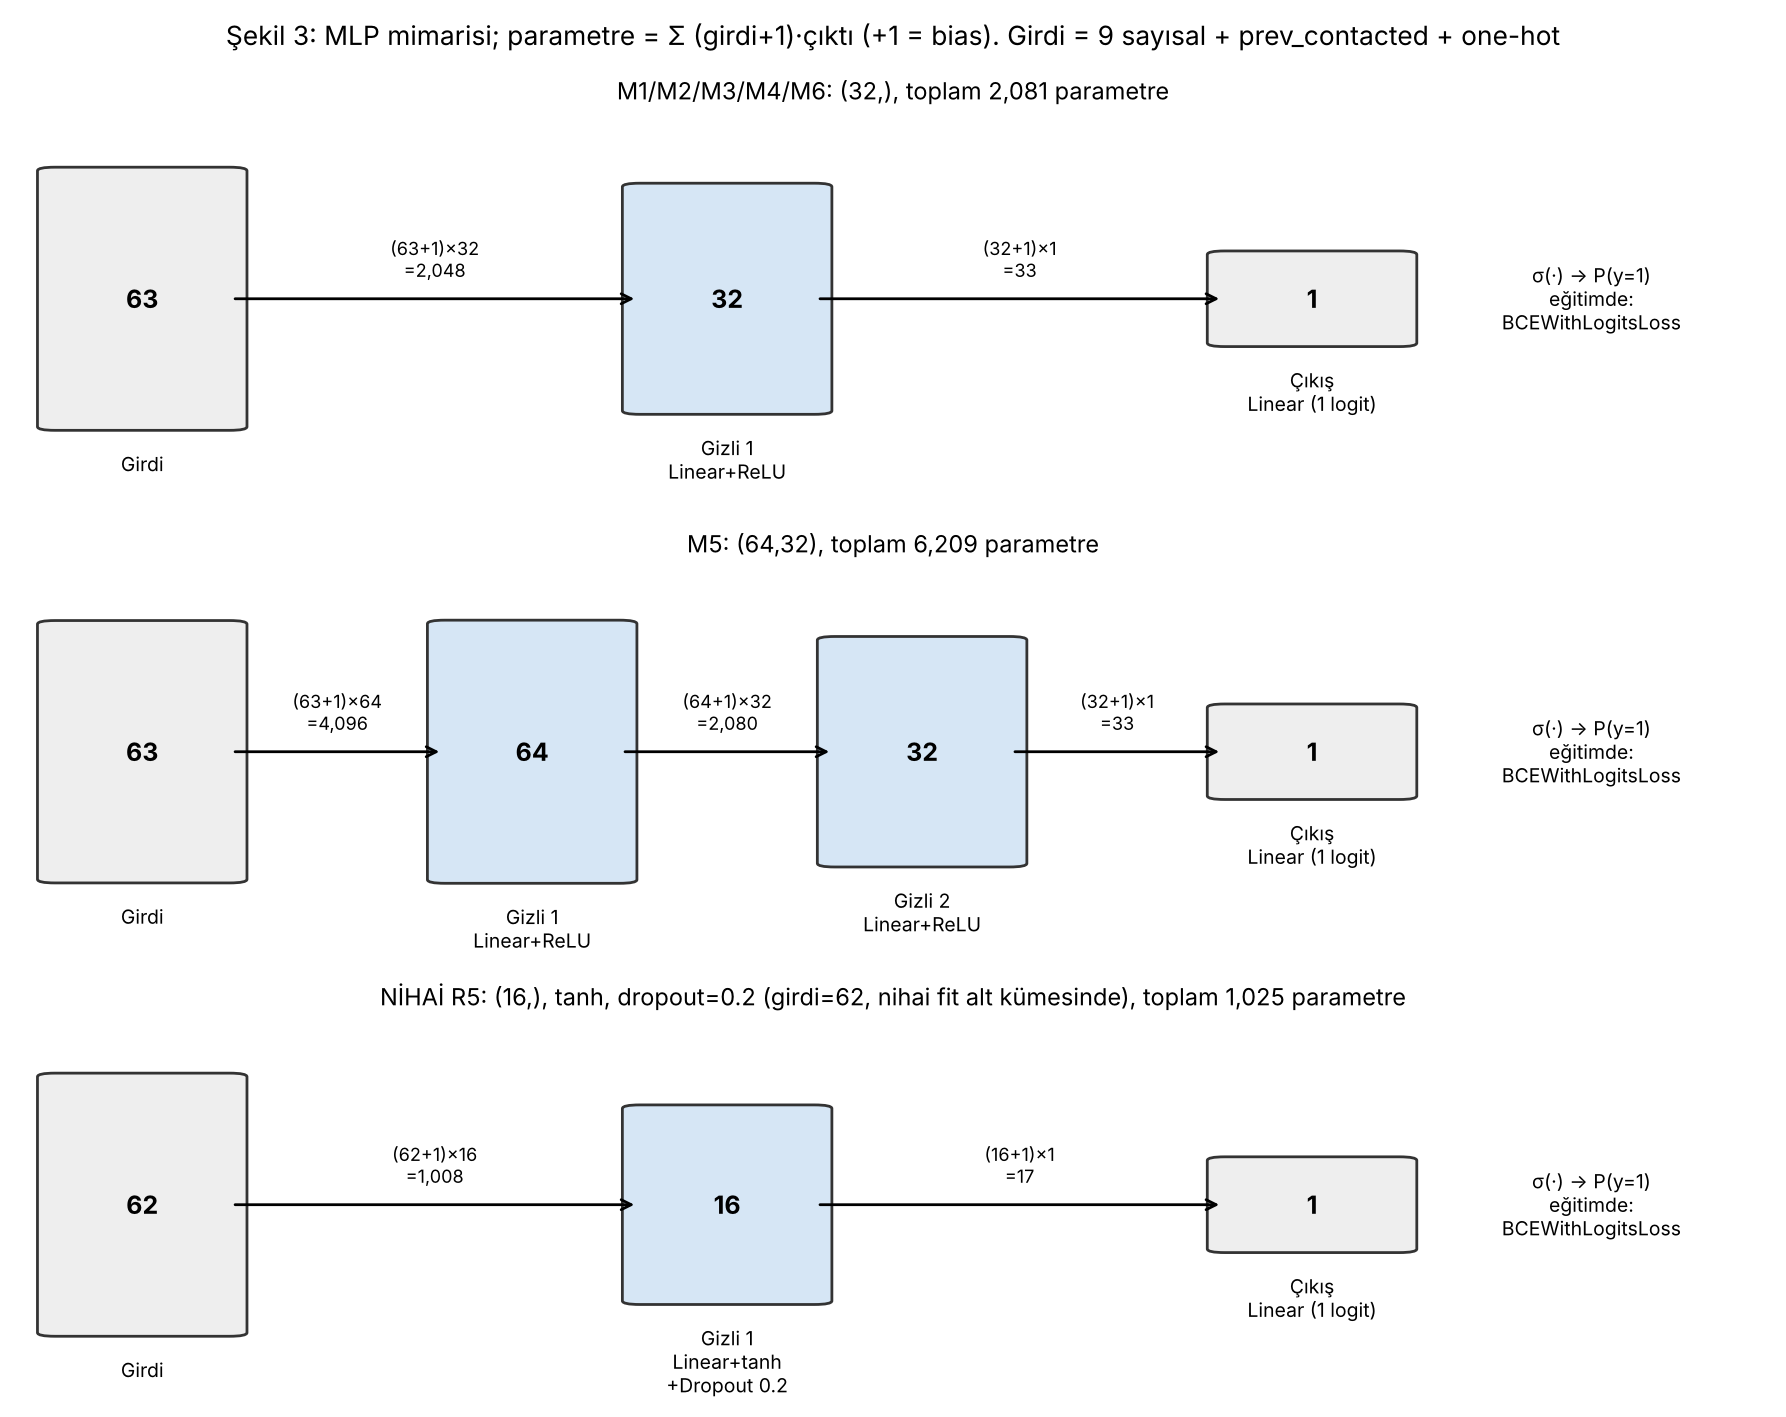
\includegraphics[width=.62\linewidth]{fig03_mlp_architecture.png}
\caption{MLP mimarileri ve parametre sayıları. Final R5 modelinde girdi sayısı 62. Parametre sayılarını (girdi + 1) x çıktı formülüyle hesaplayıp şemayı 02\_nested\_cv.ipynb içinde çizdim.}\label{fig:arch}\end{figure}

\section{Deneyler: Manuel ve Otomatik Hiperparametre Araması}
Manuel adaylar M1 modelinden tek bir ayar değiştirilerek oluşturuldu. M1: AdamW, (32,), StandardScaler, öğrenme oranı 0.001, weight decay 0.0001, scheduler açık, batch 64, dropout 0, ReLU.
Random search için ParameterSampler kullanıldı (seed 31072) ve her optimizer için 2 aday üretildi. Öğrenme oranı log ölçekte Adam ve AdamW için 0.0001-0.01, SGD için 0.001-0.1 aralığından seçildi. Diğer seçenekler: gizli katmanlar (16,), (32,), (64,), (64,32), (128,64), aktivasyon ReLU veya tanh, weight decay 0-0.001, batch 32, 64 veya 128, scaler Standard, MinMax veya Robust, dropout 0 veya 0.2, kırpma var veya yok.
12 adayın hepsi nested CV öncesinde configs klasörüne yazılıp commitlendi. Sonuçlar Tablo 3, Tablo 4, Şekil 4 ve Şekil 5 içinde.

\begin{table}[H]\centering\caption{Manuel M1-M6 adayları ve iç CV sonuçları (AP ortalama ± SD). En iyi epoch ve süre tüm development iç CV sonuçlarıdır. Değerler 02\_nested\_cv.ipynb çalışınca oluşan results/manual\_search\_results.csv dosyasından, tabloyu report/make\_tables.py ile oluşturdum.}\label{tab:manual}
\resizebox{\linewidth}{!}{\tbl{t2_manual}}\end{table}
\begin{table}[H]\centering\caption{Random search R1-R6 adayları ve iç CV sonuçları. Adayları src/make\_configs.py ile ParameterSampler kullanarak ürettim. Sonuçlar results/random\_search\_results.csv dosyasından, tablo report/make\_tables.py ile oluşturuldu.}\label{tab:random}
\resizebox{\linewidth}{!}{\tbl{t3_random}}\end{table}

\begin{figure}[H]\centering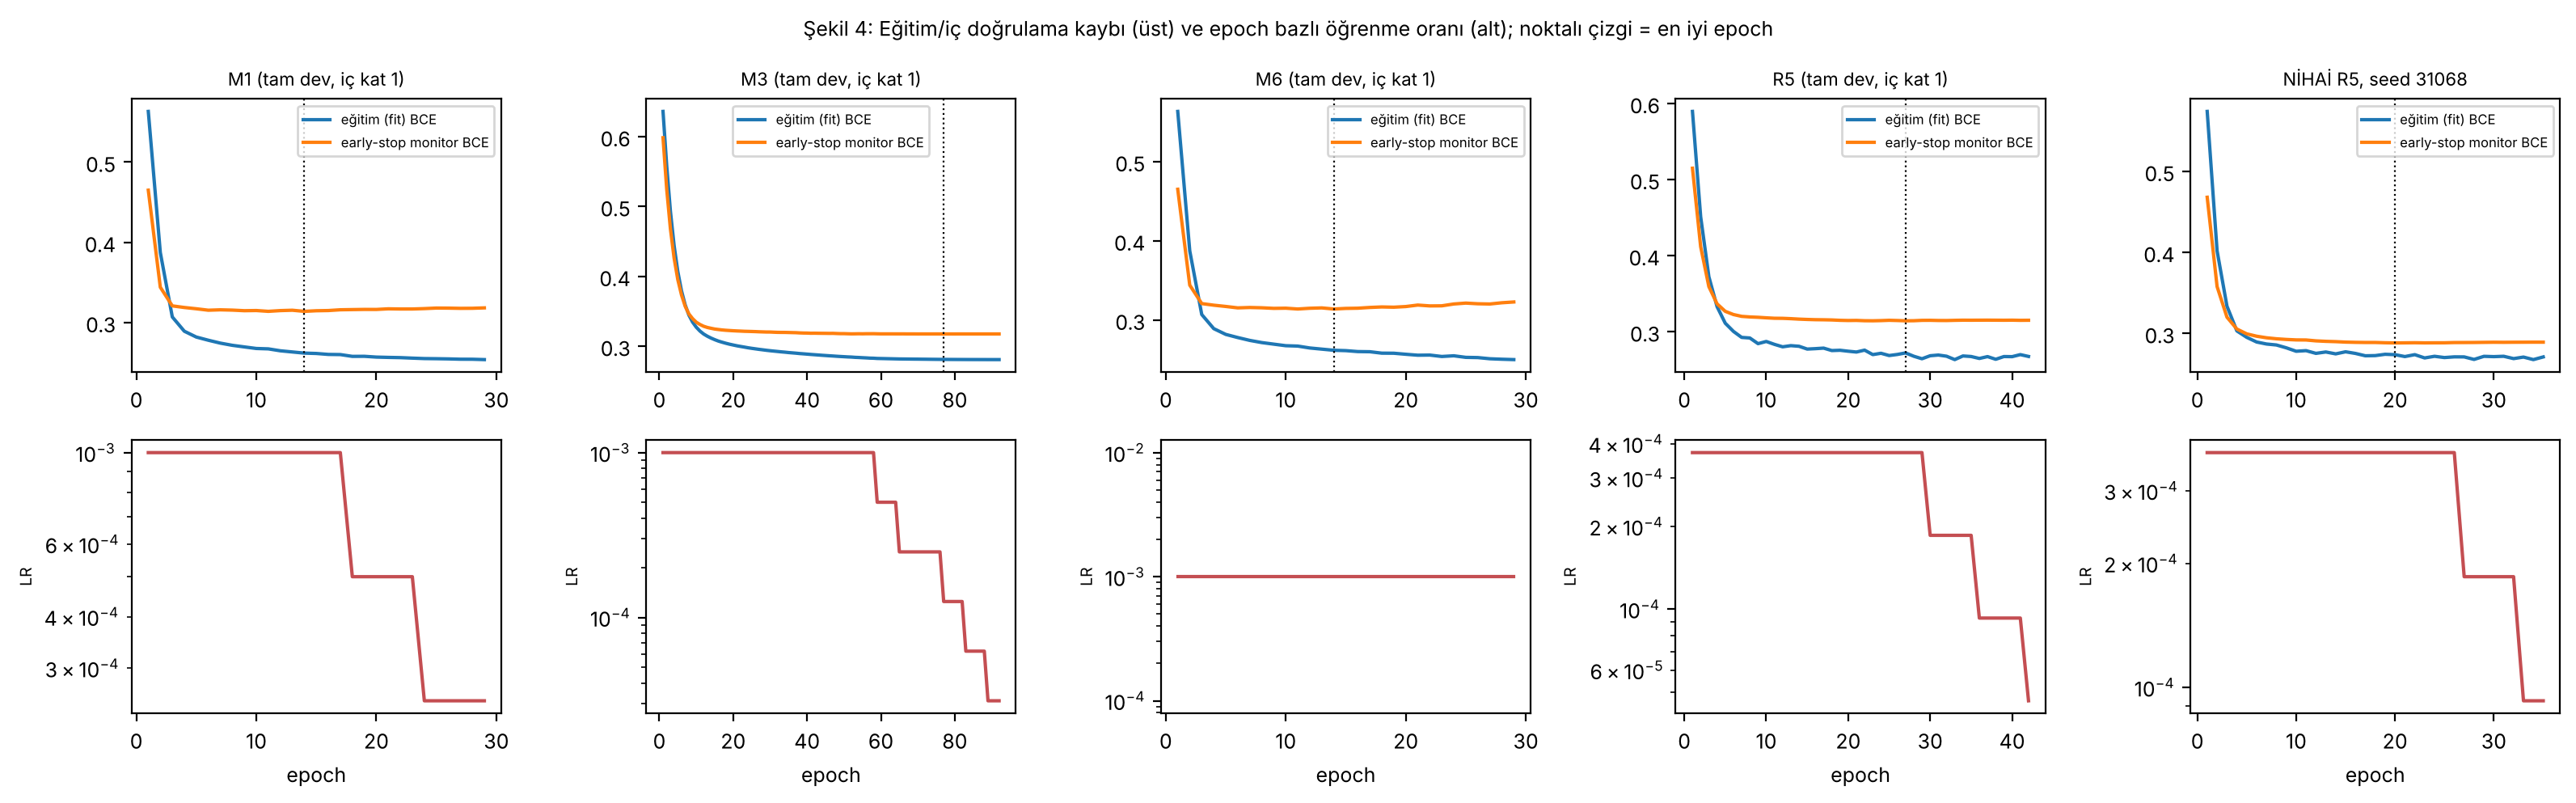
\includegraphics[width=.95\linewidth]{fig04_loss_lr_curves.png}
\caption{Eğitim ve early stopping BCE kaybı (üstte), epoch bazında öğrenme oranı (altta). Noktalı çizgi en iyi epoch. Grafiği 02\_nested\_cv.ipynb içinde eğitim sırasında kaydettiğim epoch loglarından çizdim. M1, M3 ve M6 panelleri tüm development iç CV birinci katına ait (results/training\_logs/full\_dev\_inner\_training\_logs.csv), son panel final R5 modelinin seed 31068 eğitimi (final\_model\_training\_logs.csv).}\label{fig:loss}\end{figure}
\begin{figure}[H]\centering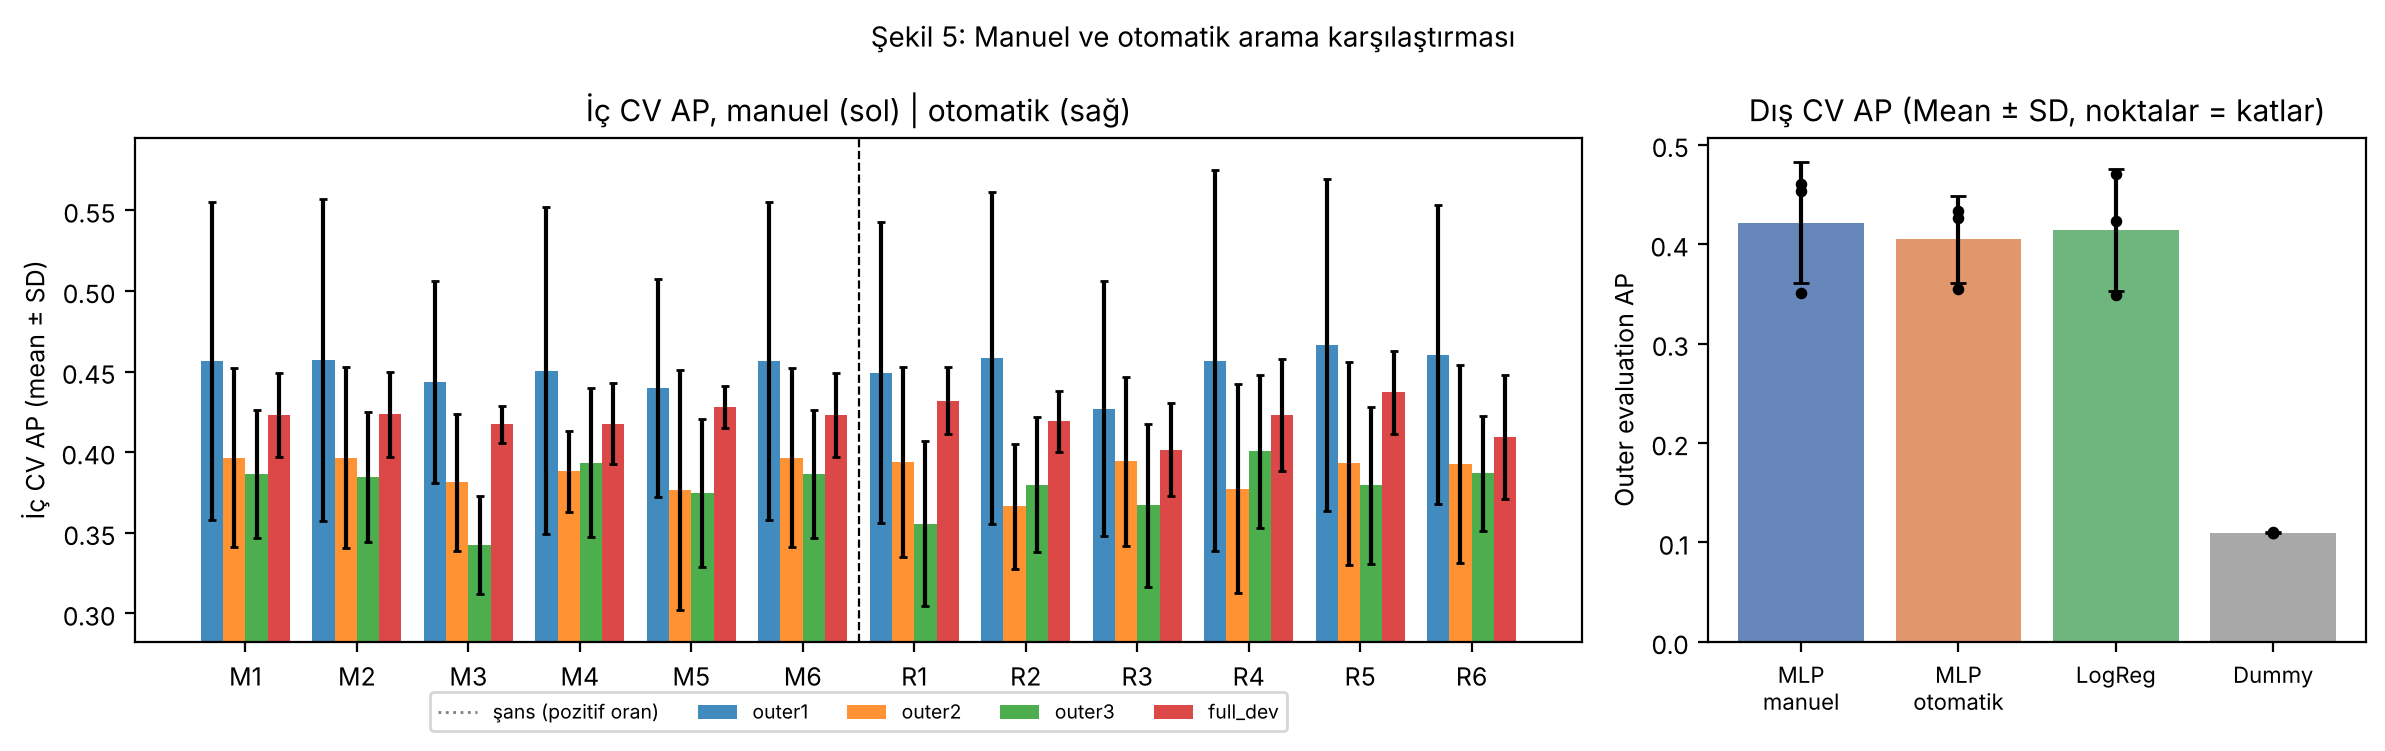
\includegraphics[width=.95\linewidth]{fig05_manual_vs_random.png}
\caption{Solda adayların iç CV AP değerleri, sağda dış CV AP ortalaması ve standart sapması. Sol paneli manual/random\_search\_results.csv, sağ paneli outer\_cv\_results.csv dosyasından 02\_nested\_cv.ipynb içinde çizdim.}\label{fig:cmp}\end{figure}

\subsection*{Hipotezlerin sonuçları}
H1 desteklendi. M3 dört aşamanın hepsinde M1 modelinden düşük AP verdi (fark 0.006-0.044). Ortalama en iyi epoch M3 için 125, M1 için 12.7 ve M3 eğitimlerinin yarısı 150 epoch sınırına takıldı. Öğrenme oranı yüksek SGD adayı R1 ise 0.432 ile en iyi ikinci aday oldu, yani sorun optimizerdan değil düşük öğrenme oranından kaynaklanıyor. Adam ile AdamW farkı her aşamada 0.002 veya daha az.
H2 kısmen desteklendi. M4 dört aşamanın üçünde M1 altında kaldı ama farklar 0.009 veya daha küçük. Kırpmanın etkisi random adaylarda diğer ayarlarla karıştığı için ayrı ölçülemedi.
H3 desteklendi. M5 üç dış katta M1 altında, tüm development üzerinde sadece 0.005 üstünde kaldı. Ortalama en iyi epoch 7 olduğu için daha erken aşırı öğreniyor.
H4 desteklendi. M6 ve M1 her aşamada birebir aynı sonucu verdi. Kayıtlara göre öğrenme oranı ilk kez en iyi epochtan 4-7 epoch sonra düşüyor ve sonrasında iyileşme olmadığı için early stopping eski ağırlıkları geri yüklüyor (Şekil 4).

\section{Nested CV Bulguları}
Dış kat sonuçları Tablo 5 ve Tablo 6 içinde. Seçilen adaylar katlara göre değişti (manuelde M2, M2, M4, random searchte R5, R3, R4), yani adaylar arası farklar iç CV dalgalanması kadar küçük.
Manuel arama 0.422 ± 0.061, random search 0.405 ± 0.044, lojistik regresyon 0.414 ± 0.061 AP verdi. Farklar katlar arası standart sapmadan çok küçük. H5 desteklendi: MLP ile LR farkı 0.01 altında ve ikisi de Dummy (0.110) modelini açıkça geçiyor.
0.50 eşiğinde sensitivity düşük (0.17-0.23), specificity yüksek (0.98-0.99), çünkü olasılıkların çoğu \%11 civarında kalıyor.
Tablo 5 içindeki son sütun AP ile trapez PR-AUC değerinin aynı olmadığını gösteriyor: Dummy için AP 0.110, trapez PR-AUC 0.555.
Üç dış kat bağımsız değil (eğitim kümeleri \%50 ortak), bu yüzden SD güven aralığı gibi yorumlanmamalı.

\begin{table}[H]\centering\caption{Dış CV kat bazlı sonuçlar (eşik 0.50). İç AP seçilen adayın iç CV ortalaması. Değerler results/outer\_cv\_results.csv dosyasından.}\label{tab:outer}
\resizebox{.92\linewidth}{!}{\tbl{t4_outer_folds}}\end{table}
\begin{table}[H]\centering\caption{Dış CV özeti, ortalama ± örnek standart sapma (3 kat). outer\_cv\_results.csv üzerinden pandas std(ddof=1) ile hesapladım.}\label{tab:outerms}\small
\tbl{t5_outer_meansd}\end{table}

Son seçimde tüm development iç CV sonucu manuel aramada M5 (0.428), random searchte R5 (0.437) oldu ve kurala göre R5 seçildi: AdamW, (16,), tanh, öğrenme oranı 0.00037, weight decay 0, batch 32, StandardScaler, dropout 0.2, 1025 parametre. Dış CV sonucunda manuel arama biraz daha iyi görünse de karar değiştirilmedi, çünkü dış sonuçlara göre seçim yapmak bu sonuçları tarafsız ölçüm olmaktan çıkarırdı.

\section{Bağımsız Test}
R5 tüm development ile 3 seed kullanılarak eğitildi (2800 fit, 495 early stopping gözlemi, en iyi epoch 20, 23 ve 19). Test tahminleri etiketlere bakılmadan kilitlendikten sonra 03 notebook etiketleri okudu (Tablo 7, Şekil 6, Şekil 7).
Ana model 0.440 AP (\%95 CI 0.336-0.561), 0.784 ROC-AUC (0.727-0.843) ve 0.331 F1 (0.213-0.433) aldı. Lojistik regresyon 0.437 AP ve 0.793 ROC-AUC verdi.
Eşleştirilmiş bootstrap ile AP farkı +0.003 (-0.020 ile +0.023), ROC-AUC farkı -0.009 (-0.032 ile +0.012) çıktı. İkisi de sıfırı içerdiği için anlamlı fark yok. Bootstrap örneklerinin hiçbirinde tek sınıf oluşmadı.
Üç seed ile test AP 0.432 ± 0.007 (Tablo 8). Ana seed en yüksek değeri verdi ama baştan belirlendiği için ana sonuç olarak kullanıldı.

\begin{table}[H]\centering\caption{Bağımsız test sonuçları (eşik 0.50) ve bootstrap \%95 güven aralıkları. 03\_final\_test.ipynb içinde kilitli tahmin dosyasından hesapladım (test\_metrics.csv, test\_bootstrap\_ci.csv).}\label{tab:test}
\resizebox{\linewidth}{!}{\tbl{t6_test}}\end{table}
\begin{table}[H]\centering\caption{Üç ağırlık seed değeri ile test sonuçları. 03\_final\_test.ipynb içinde hesapladım (seed\_stability\_results.csv).}\label{tab:seed}\small
\resizebox{.9\linewidth}{!}{\tbl{t7_seeds}}\end{table}

\begin{figure}[H]\centering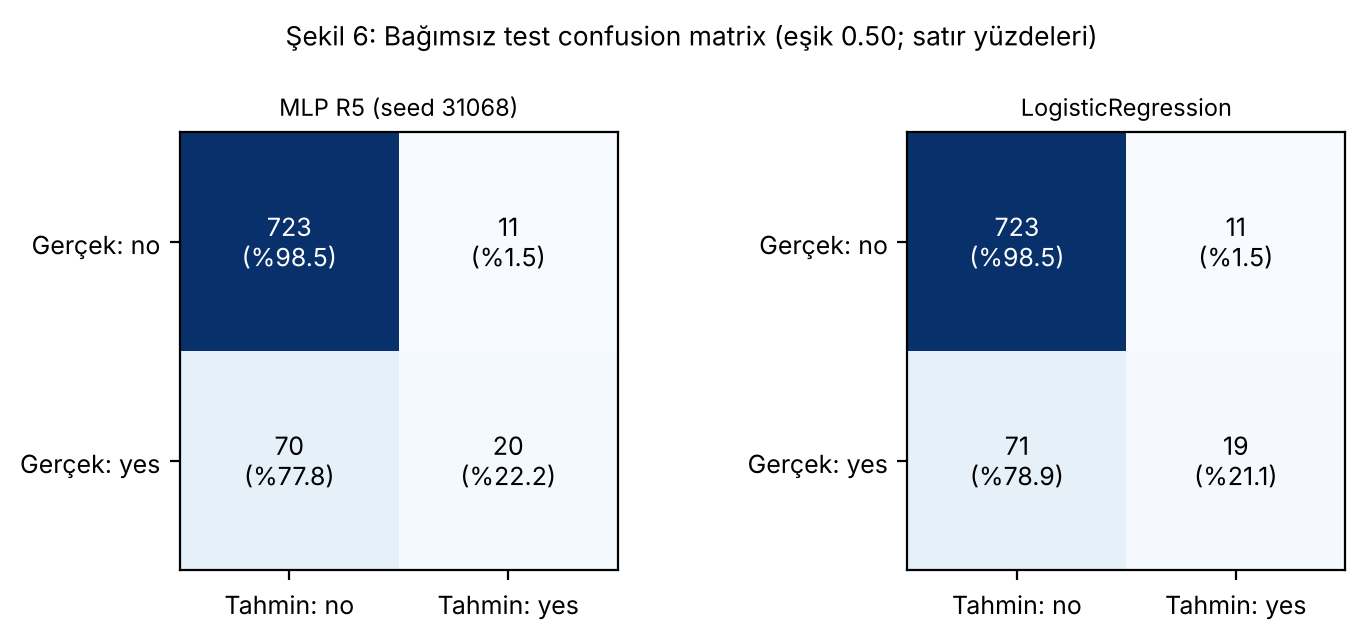
\includegraphics[width=.55\linewidth]{fig06_confusion_matrices.png}\caption{Test confusion matrix (MLP ve LR, eşik 0.50). 03\_final\_test.ipynb içinde kilitli tahminlerden çizdim.}\label{fig:cm}\end{figure}
\begin{figure}[H]\centering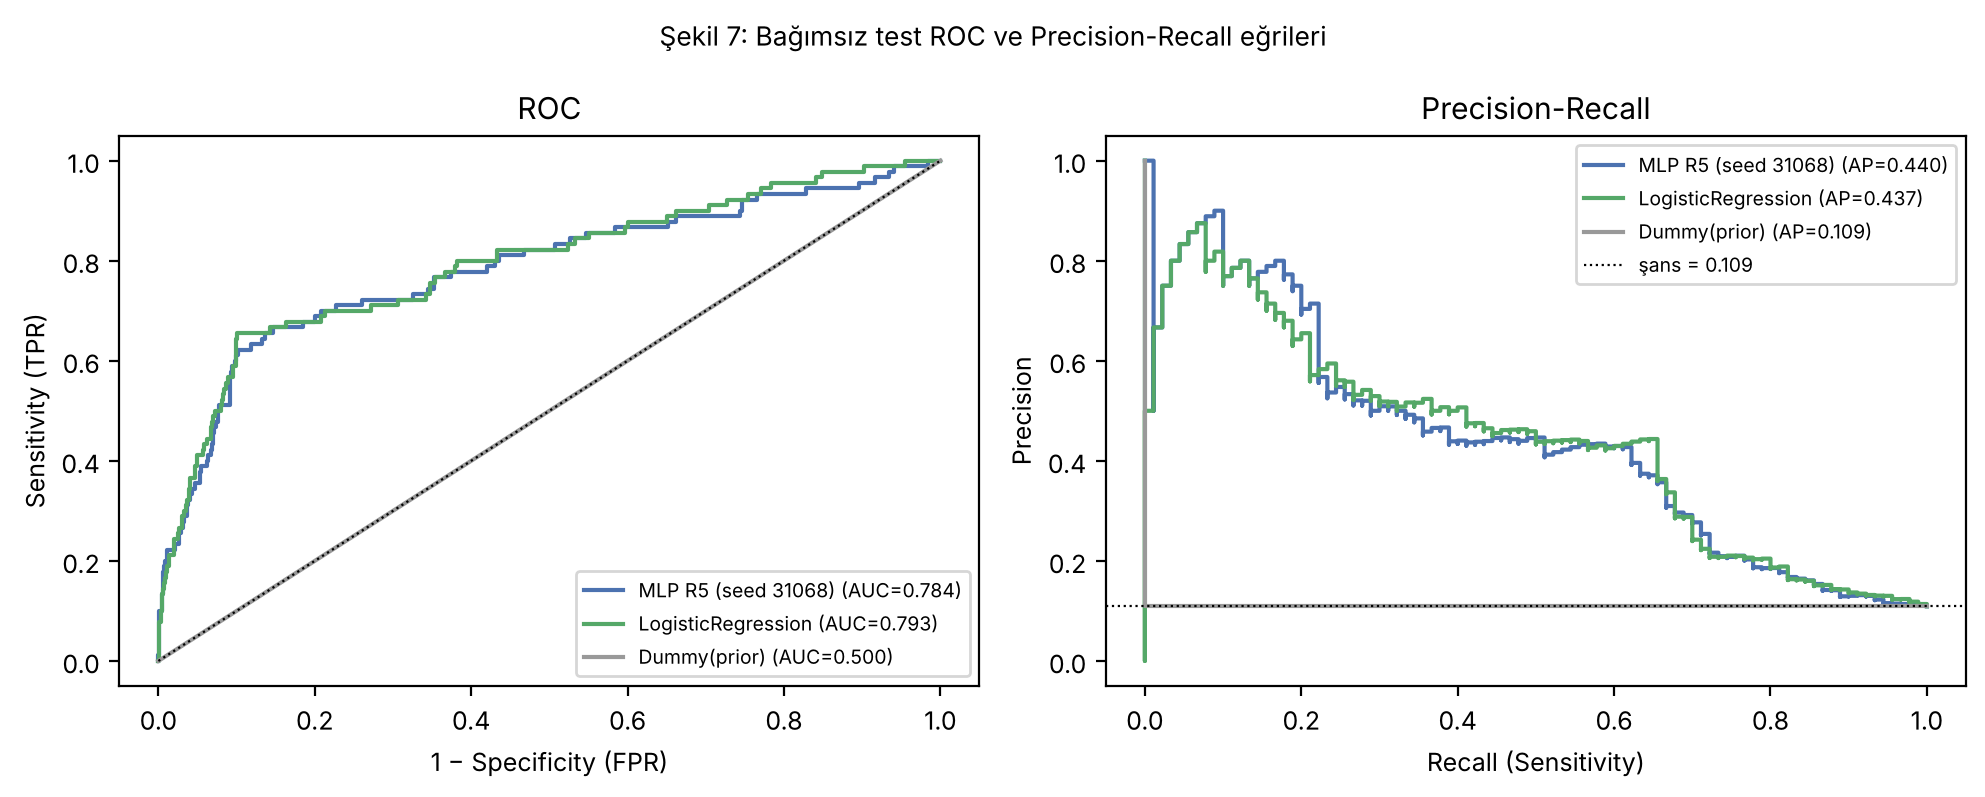
\includegraphics[width=.85\linewidth]{fig07_roc_pr_curves.png}\caption{Test ROC ve Precision-Recall eğrileri. 03\_final\_test.ipynb içinde scikit-learn roc\_curve ve precision\_recall\_curve ile çizdim.}\label{fig:roc}\end{figure}

\section{Tartışma}
Dış CV sonucu 0.405 ± 0.044 iken R5 için tüm development iç CV skoru 0.437. İkincisi 12 aday arasından en iyisi seçildiği için biraz iyimser. Test sonucu (0.440, üç seed ortalaması 0.432) dış CV sonucundan biraz yüksek ama geniş güven aralığının içinde. Final modelin daha fazla veriyle eğitilmesi (3295 ve 2197) ve testte sadece 90 pozitif olması bu farkı açıklayabilir. Gerçekçi AP değeri 0.40-0.44 civarında görünüyor.

Optimizer açısından ortalama eğitim süresi Adam için 0.26, AdamW için 0.27, SGD için 0.46 saniye oldu. SGD ortalama 84. epoch civarında dururken Adam 22. ve AdamW 28. epoch civarında durdu. Yani aday sayısı eşit olsa da harcanan süre eşit değil.
Büyük modeller (R6 16513, R4 ve M5 6209 parametre) 3-10 epoch içinde en iyi noktaya ulaşıp sonra aşırı öğrenmeye başladı. En iyi sonuç küçük, dropout kullanan ve düşük öğrenme oranlı R5 modelinden geldi.
MLP doğrusal modeli geçemedi çünkü duration olmadan bilginin büyük kısmı birbiriyle çok yüksek korelasyonlu ekonomik göstergelerde ve önceki kampanya sonucunda kalıyor. Bu yapıyı lojistik regresyon da iyi öğrenebiliyor.

Hata analizinde (Tablo 9) ana model 90 pozitifin 20 tanesini buldu. 70 false negative ve 11 false positive var. Doğru bulunan pozitiflerin \%90 kadarının önceki kampanyası başarılıyken false negativelerde bu oran \%2.9. Yani model pozitifleri büyük ölçüde önceki kampanya başarısından tanıyor ve ilk kez aranıp abone olanları ayırt edemiyor. False negativelerin medyan olasılığı 0.153, yani model doğru yönde ama 0.5 eşiğinin altında kalıyor. Daha fazla pozitif yakalamak istenirse eşik sadece development iç CV tahminleriyle seçilmeli.
Ek olarak Brier skoru MLP için 0.0781, LR için 0.0776 çıktı. unknown değerlerini en sık değerle doldurmak R5 için iç CV sonucunu değiştirmedi (0.437 ve 0.439). Kalibrasyon ve eşik grafikleri figures klasöründe var, seçim için kullanılmadı.

\begin{table}[H]\centering\caption{Test hata analizi (ana MLP, eşik 0.50). 03\_final\_test.ipynb içinde hesapladım (test\_error\_analysis.csv).}\label{tab:err}\small
\resizebox{.9\linewidth}{!}{\tbl{t8_errors}}\end{table}

Sınırlamalar: Rastgele bölünme zamansal genellemeyi göstermiyor. Test seti küçük olduğu için güven aralıkları geniş. 3 dış kat belirsizliği kabaca gösteriyor. Her aramada sadece 6 aday olduğu için seçim iç CV dalgalanmasına duyarlı. Test etiketleri açık olduğu için kilitli commit tam kör test değil, sadece sırayı gösteriyor. 144 iç eğitimin 16 tanesinde uyarı oluştu (6 tanesi M3 için 150 epoch sınırı, diğerleri çok erken en iyi epoch). Donanım 2 çekirdekli CPU, nested CV yaklaşık 35 saniye sürdü.

\section{Sonuç}
3x3 nested CV ile 6 manuel ve 6 random MLP adayı sızıntı olmadan karşılaştırıldı ve süreç seedler sayesinde tekrar üretilebilir. Düşük öğrenme oranlı SGD yavaş öğrendi (H1), MinMax biraz geride kaldı (H2), büyük model kazanç getirmedi (H3) ve early stopping varken scheduler etkisiz kaldı (H4). Final R5 modeli testte 0.440 AP aldı ama lojistik regresyondan anlamlı şekilde ayrışmadı (H5). Bu veride başarıyı model türünden çok verideki bilginin sınırlı olması belirliyor.

\section*{Kaynakça}
\small
\begin{enumerate}[label={[\arabic*]}]
\item Moro, S., Rita, P. ve Cortez, P. (2014). Bank Marketing. UCI Machine Learning Repository. \url{https://doi.org/10.24432/C5K306}
\item scikit-learn. Common pitfalls and recommended practices. \url{https://scikit-learn.org/stable/common_pitfalls.html}
\item scikit-learn. Cross-validation, model selection ve metrics belgeleri. \url{https://scikit-learn.org/stable/}
\item PyTorch. ReduceLROnPlateau. \url{https://docs.pytorch.org/docs/stable/generated/torch.optim.lr_scheduler.ReduceLROnPlateau.html}
\item Cawley, G. C. ve Talbot, N. L. C. (2010). On Over-fitting in Model Selection and Subsequent Selection Bias in Performance Evaluation. JMLR, 11, 2079-2107.
\end{enumerate}
\end{document}
